\subsection{What is continuous integration?}

Continuous integration(CI) is a technique for building software incrementally, as in a way
to automate the build and testing of the code. This method encourages developers to 
write code that is more readable, more maintainable, and more testable. Also it makes
it easier to find bugs before they are introducted into the main code, and to
catch as much problems as possible before the code reaches the production environment.

CI has emerged as a great tool for software development, as it eases the process of
merging code from different branches which allows for a more efficient development process,
as developers mostly work on their own branch in isolation, and this allows them to 
introduce features and fixes that integrate with the rest of the code. \cite{ci_msft}

Along with CI, there is Continuous Delivery(CD), which is the other end of this process
and is used to push code to a production environment, allowing for smoother introduction
of updates, hotfixes, \dots

\subsection{CI/CD projected on the system}

As one of the most important features within the industrialization of the project
was having a reliable and maintainable deployment process, here where came the 
continuous intagration pipelines. The CI pipeline offered a great way to have
a reliable and maintainable deployment process and to automate the whole process
of the project.

\begin{figure}[!htpb]
    \centering
    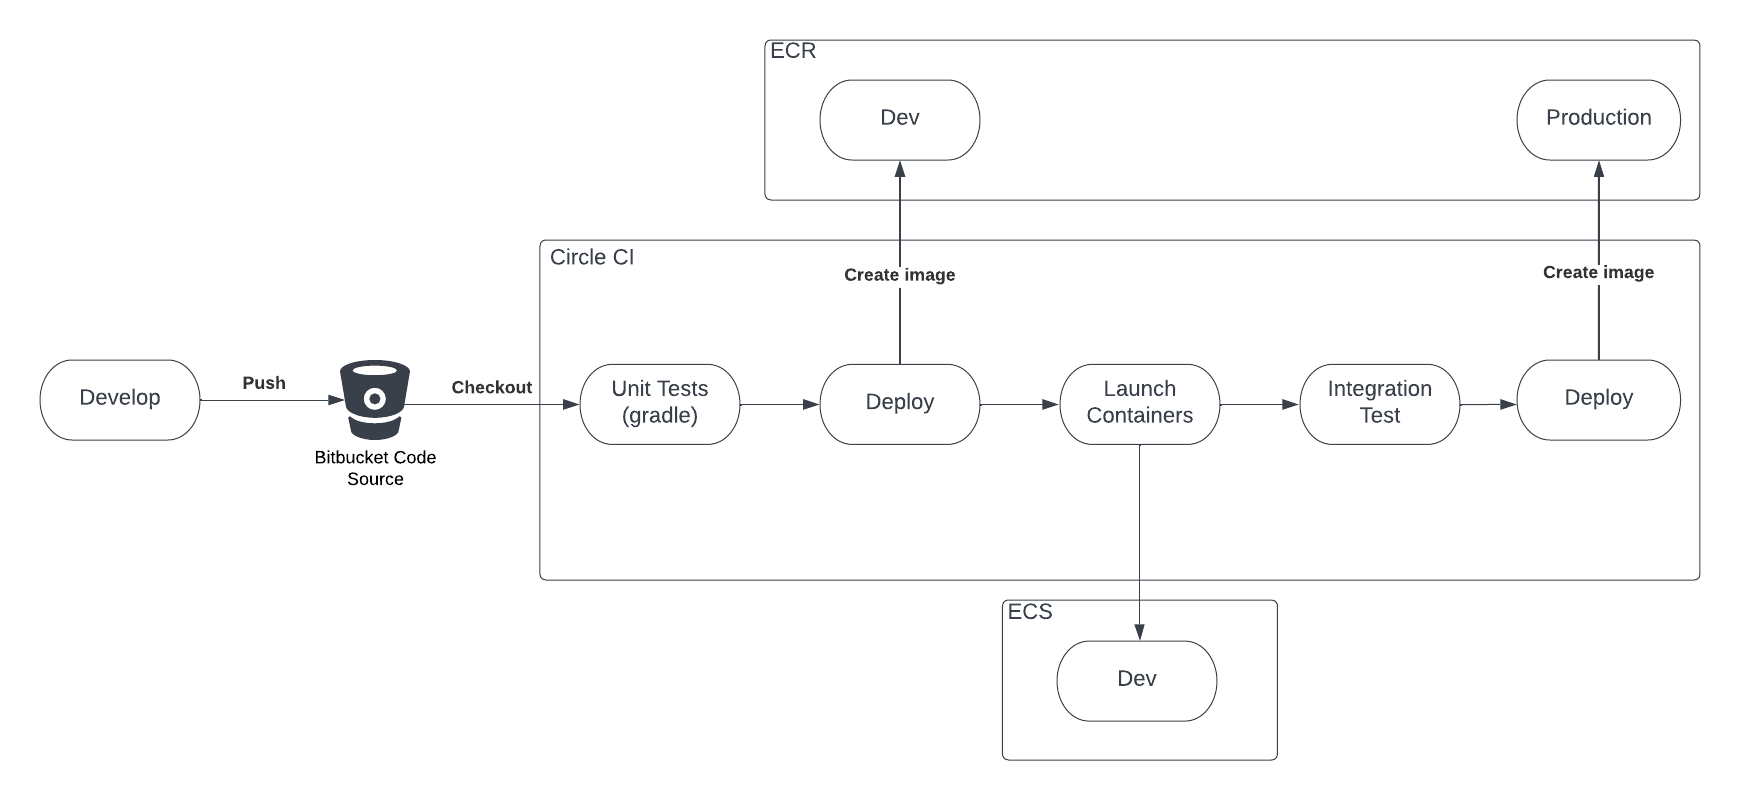
\includegraphics[width=\textwidth]{images/ci-cd-pipeline.png}
    \caption{Continuous integration pipeline}
    \label{fig:ci-cd-pipeline}
\end{figure}

As shown in the figure \ref{fig:ci-cd-pipeline}, the CI pipeline is composed
of three main steps:
    \begin{itemize}
        \item \textbf{Test}: the test phase is the first step of the CI pipeline.
            It is responsible for running the tests built on the project using
            the gradle test task.
        \item \textbf{Coverage}: the coverage phase is the second step of the CI pipeline.
            It uses SonarScanner, which is a scanner for code analytics reporting things
            from code quality to security threats. It generates the coverage report of the
            project and then it sends the report to the SonarCloud\footnote{SonarCloud is
                a cloud service used for hosting SonarQube scans} server.
        \item \textbf{Build and Deploy}: the build and deploy phase is the last step
            of the CI pipeline. It is responsible for building a docker image and then
            pushing it to ECR (EC Container Registry) and then deployed to ECS
            (ECS Container Service) all that using a range of custom scripts built
            by us within gradle, to ease up the deployment within the pipeline.
    \end{itemize}

The CI/CD service we've went for was the Circle CI, which is a hosted continuous
integration service that is used to test the code and to deploy the application.
The configuration of the CI/CD service was configured within a yaml file,
which is located in the \texttt{.circleci/config.yml} file.

The test and building steps both came from taking advantage of the gradle build
system, which were already setup and configured within the project. But nonetheless,
as the CI/CD pipeline creates docker containers to run the tests and the build,
and the tests needed AWS credentials to be able to run, we had to somehow pass
the file containing the AWS credentials to the CI/CD pipeline, which was done
by creating new AWS credentials creating a AWS credentials file then encoding to
base64 and passing it to the CI/CD pipeline as a environment variable, then decoding
it to a string to be stored in the \texttt{.aws/credentials} inside the pipeline which
was a play around to pass the files to any virtualized environment not allowing for 
those accesses.

Next came the coverage phase, which was a bit more involved. The coverage takes care
of analyzing the code to see if there are any security issues, bugs, bad code and
everything that relate to code analysis, and then it sends the report to the
SonarCloud server. The important thing in this phase is that it can be as a test to
the code's quality, so you can set the threshold of the coverage to be a certain
percentage, and if the coverage is below that threshold, then the CI/CD pipeline
will fail so we can stop critical issues from being deployed if they weren't caught
during development.

The deployment, which is the last step of the CI pipeline, is done using orbs
within Circle CI, orbs are snippets of codes used to automate repeatable processes
and published by the Circle CI team, specifically the ECR and ECS orbs.

As the orbs didn't come in handy, as we had different way of building the docker image
than the default one, we opted to creating our own job within the CI/CD pipeline
which took care of the building and deployment phase of the project.
The job went as follow: 
    \begin{itemize}
        \item Create a docker image using the gradle build tool.
        \item Tag the docker image with the project name.
        \item Push the docker image to ECR.
        \item Set ECR image with the right tags.
        \item Restart the ECS running tasks to run the new image.
    \end{itemize}

In the end, the CI/CD pipeline was configured to only build and deploy on two branches
which are "master" to deploy on the production environment and "dev" to deploy on the
development environment.
